\chapter{ANTECEDENTES}\label{cap:antecedentes}
\listasdecapitulo{1}

El control adaptativo de sistemas semafóricos es un campo con décadas de desarrollo. A nivel mundial han
surgido enfoques que ajustan en tiempo real la duración de las fases en función de la demanda detectada,
como SCATS (Sídney) y SCOOT (Reino Unido), o que distribuyen la decisión por intersección y coordinan
planes con los cruces vecinos, como Surtrac (Universidad Carnegie Mellon). Estas experiencias evidencian
que la semaforización adaptativa puede reducir la congestión, mejorar la velocidad promedio y disminuir las
demoras y las emisiones. En América Latina se observa un interés creciente por modernizar la gestión del
tránsito, y en el Perú destaca el caso del distrito de San Isidro, donde en 2024 se renovaron varias
intersecciones con semáforos inteligentes interconectados a un centro de control municipal
(Figura~\ref{fig:san-isidro}). El estado del arte detallado de estos sistemas se desarrolla en el
Capítulo~\ref{cap:estado-arte}.

\begin{figure}[H]
  \centering
  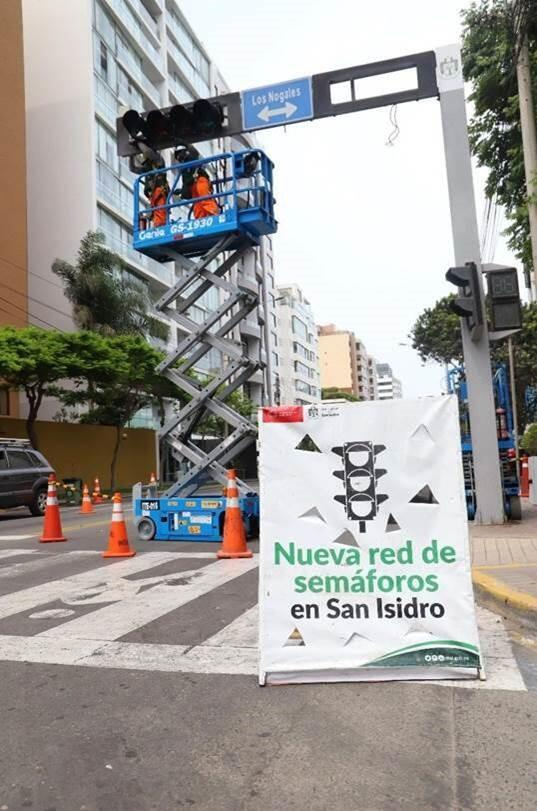
\includegraphics[width=0.85\linewidth,keepaspectratio]{media/image149.png}
  \caption{Instalación de semáforos inteligentes en San Isidro, dentro del proyecto de modernización de la
  red semafórica en Lima.}
  \label{fig:san-isidro}
  \fuente{ITS Perú (2024).}
\end{figure}

La experiencia local confirma la factibilidad técnica y los beneficios de adoptar semaforización adaptativa
con tecnología moderna. Al mismo tiempo, la digitalización de la infraestructura vial introduce una
preocupación de ciberseguridad: los controladores, antes dispositivos aislados, quedan expuestos a riesgos
propios de cualquier equipo conectado. Diversos estudios han documentado vulnerabilidades en equipos de
semaforización existentes, lo que obliga a considerar la seguridad cibernética desde la definición de la
arquitectura.

\section{Descripción de la problemática}\label{sec:problematica}

La congestión de Lima Metropolitana constituye el contexto urbano; sin embargo, el problema que aborda esta
tesis es específicamente técnico. Una parte de las intersecciones opera con planes de tiempo fijo o con
adaptación limitada, de modo que una distribución de verde calculada para una demanda nominal permanece
activa aun cuando cambian el flujo, la dirección dominante o la longitud de cola. Como consecuencia, pueden
coexistir accesos saturados con otros subutilizados. Esta limitación reduce la capacidad efectiva de la
intersección y dificulta responder a variaciones que ocurren en una escala temporal menor que la
actualización manual de los planes.

La adaptación requiere sensado local, porque la variable que debe corregirse —la demanda efectiva en cada
acceso— no puede inferirse únicamente a partir del horario programado. Una cámara permite estimar conteo,
velocidad, ocupación y cola sin intervenir el pavimento; no obstante, su información debe procesarse cerca
de la intersección para reducir latencia, limitar el envío continuo de video y mantener la operación cuando
la conexión externa se degrada. En consecuencia, el procesamiento en el borde no se adopta solo por
conveniencia informática, sino como requisito de disponibilidad del lazo de decisión.

La nube aporta almacenamiento histórico, supervisión remota, coordinación entre intersecciones, gestión de
configuraciones y análisis de tendencias, pero no debe ser indispensable para las decisiones críticas de
cada ciclo: la red celular o el enlace con el centro de control pueden presentar latencia, pérdida de
paquetes o indisponibilidad, y una arquitectura exclusivamente centralizada convertiría la conectividad en
un punto único de falla. Por ello, ante pérdida de enlace, el módulo debe continuar estimando el tráfico y
generando recomendaciones locales acotadas, mientras el controlador semafórico conserva el plan seguro y la
autoridad final de actuación.

La incorporación de comunicaciones bidireccionales introduce riesgos de acceso no autorizado, manipulación
de parámetros, inyección de datos falsos, denegación de servicio y compromiso de credenciales. La
ciberseguridad forma parte del diseño porque una recomendación alterada o una telemetría falsa puede
degradar la operación vial incluso sin acceso directo a las lámparas. La separación entre recomendación y
actuación, la autenticación, el cifrado, la validación de rangos, el registro de eventos y el modo local
seguro reducen este riesgo, sin atribuir al presente trabajo una certificación que no ha sido ejecutada.

La pertinencia para Lima se sustenta en la heterogeneidad de la infraestructura, la existencia de
intersecciones aisladas o con coordinación limitada, la dificultad de desplegar obras civiles extensas y la
necesidad de una modernización progresiva. La Figura~\ref{fig:arbol-problemas} resume las causas y los
efectos del problema. Un módulo complementario permite plantear una integración gradual y reversible, sujeta
a la compatibilidad con el controlador instalado y a las autorizaciones municipales. Por lo tanto, la
necesidad técnica se formula de la siguiente manera: \textbf{diseñar un módulo IoT mecatrónico,
complementario al controlador semafórico existente, capaz de estimar el estado de congestión local, ajustar
parámetros de control mediante lógica difusa, comunicar datos a una plataforma en la nube y operar bajo
criterios mínimos de seguridad, disponibilidad y ciberseguridad}.

\begin{figure}[H]
  \centering
  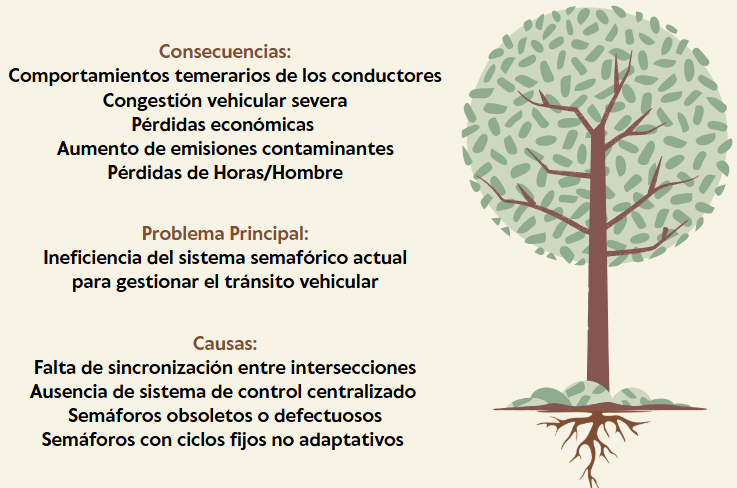
\includegraphics[width=0.9\linewidth,keepaspectratio]{media/image116.png}
  \caption{Árbol de problemas de la gestión semafórica en intersecciones de Lima.}
  \label{fig:arbol-problemas}
  \fuente{Elaboración propia.}
\end{figure}

\section{Propuesta de solución}\label{sec:propuesta}

Se propone diseñar un módulo IoT complementario por intersección. La cámara constituye el sensor principal;
el procesamiento local extrae variables de tráfico y calcula un índice de congestión; el controlador difuso
transforma dichas variables en ajustes recomendados de tiempo de verde dentro de límites mínimos, máximos y
de despeje. Estas recomendaciones se entregan por una interfaz definida y deben ser aceptadas, rechazadas o
acotadas por el controlador semafórico o por la central autorizada. La propuesta no conecta una salida de
propósito general directamente a las lámparas.

La plataforma en la nube recibe telemetría, estados, alertas y registros; conserva históricos y puede emitir
parámetros de configuración o recomendaciones de coordinación previamente autorizados. La operación local no
depende de una respuesta de la nube: si se pierde conectividad, el módulo conserva la última configuración
válida, registra eventos localmente y continúa en modo degradado; si el sensado pierde calidad, deja de
generar ajustes adaptativos y solicita el retorno al plan base del controlador.

La solución se valida como diseño mecatrónico mediante requerimientos trazables, selección de alternativas,
cálculos de alimentación y protección, diseño de gabinete y soporte, definición del control difuso, análisis
de amenazas y comparación reproducible en SUMO. El aporte demostrable es, por tanto, una arquitectura de
modernización gradual y un procedimiento de verificación; cualquier mejora de tráfico se sustenta con los
resultados cuantitativos obtenidos en los escenarios de simulación (Capítulo~\ref{cap:validacion}).

\section{Objetivos de la tesis}\label{sec:objetivos}

\subsection{Objetivo general}

Diseñar y validar en un entorno simulado y controlado un módulo IoT complementario para el control
semafórico adaptativo en intersecciones urbanas, integrando sensado vehicular, procesamiento local, lógica
difusa, comunicación segura con la nube y criterios de ciberseguridad, manteniendo al controlador semafórico
existente como autoridad final de seguridad funcional.

\subsection{Objetivos específicos}

\begin{enumerate}[label=\textbf{OE\arabic*:},leftmargin=1.7cm]
\item Revisar el estado del arte de control semafórico, sensado vehicular, procesamiento en el borde,
comunicaciones IoT, nube, ciberseguridad y simulación, y consolidar las decisiones de diseño derivadas en
una tabla de criterios adoptados.
\item Definir requerimientos funcionales, electrónicos, mecánicos, de control, comunicación, operación,
mantenimiento, ciberseguridad, validación y costo, indicando para cada uno su criterio y método de
verificación.
\item Desarrollar el diseño conceptual mediante caja negra, entradas y salidas, estructura funcional por
dominios, matriz morfológica y evaluación técnico-económica de alternativas, hasta seleccionar una
arquitectura trazable.
\item Diseñar el subsistema electrónico del módulo IoT, justificando sensores, unidad de procesamiento,
interfaces, comunicaciones, alimentación, protecciones, diagnóstico y respaldo energético mediante esquemas,
cálculos y tablas de selección.
\item Diseñar el subsistema mecánico —gabinete modular, distribución interna, protección ambiental, acceso
de mantenimiento y soporte o movimiento de cámara— y verificarlo mediante CAD, cálculos y análisis
estructural y térmico.
\item Diseñar el control adaptativo local basado principalmente en lógica difusa, definiendo entradas,
salida, funciones de pertenencia, reglas, inferencia, defuzzificación, restricciones de fase y modos
degradados.
\item Diseñar la arquitectura de comunicación y nube para telemetría, históricos, alertas, coordinación y
actualización autorizada de parámetros, demostrando que la decisión local puede continuar sin conectividad
externa.
\item Diseñar una arquitectura de ciberseguridad mediante modelo de amenazas, autenticación, cifrado,
control de acceso, validación de parámetros, registro de eventos y principio de mínimo privilegio.
\item Validar en SUMO el núcleo de control mediante escenarios reproducibles que comparen, como mínimo,
control fijo y control difuso adaptativo, reportando tiempo de espera, colas, velocidad, throughput,
paradas, índice de congestión y, cuando esté disponible, consumo o emisiones.
\item Elaborar un análisis económico preliminar de CAPEX y OPEX por intersección, diferenciando costos del
módulo local, conectividad, nube, mantenimiento y etapas posteriores de certificación o piloto.
\end{enumerate}

\section{Alcance del trabajo}\label{sec:alcance}

El presente trabajo corresponde a una tesis de diseño mecatrónico enfocada en el diseño, la simulación y la
validación en entorno controlado de un módulo IoT complementario para el control semafórico adaptativo.
Incluye: diseño conceptual; especificación de requerimientos; arquitectura funcional; diseño electrónico y
mecánico; arquitectura de comunicación y nube; arquitectura de ciberseguridad; algoritmo de control difuso
local; integración con una plataforma controlada de supervisión; simulación comparativa en SUMO; y análisis
económico preliminar CAPEX/OPEX por intersección.

El sistema se plantea como una solución de apoyo al controlador semafórico existente. Por tanto, el
controlador certificado de la intersección mantiene la autoridad final sobre los estados de luces,
enclavamientos, fases incompatibles y modos seguros. El módulo propuesto calcula variables de tráfico,
genera recomendaciones o parámetros de ajuste y comunica información hacia la nube y la central semafórica,
sin sustituir los mecanismos de seguridad funcional propios del controlador vial.

El trabajo no incluye fabricación física, instalación en vía pública, certificación de seguridad funcional,
auditoría formal de ciberseguridad, pruebas con tráfico real, integración certificada con controladores
comerciales específicos ni despliegue metropolitano completo. La compatibilidad con marcas y protocolos
presentes en Lima se formula como una arquitectura de integración y debe verificarse posteriormente con
equipos propietarios. Del mismo modo, la referencia a la norma IEC 62443 y a buenas prácticas de seguridad
expresa criterios de diseño, no conformidad certificada. Estas exclusiones corresponden a etapas posteriores
de madurez tecnológica: fabricación de prototipo, banco de integración \textit{hardware-in-the-loop}, piloto
controlado, evaluación normativa y certificación.

\section{Metodología empleada}\label{sec:metodologia}

Para el desarrollo de la tesis se emplea la VDI 2221 como marco principal de diseño sistemático y la VDI
2206 para ordenar la integración y verificación de los dominios mecánico, electrónico, de control y
software. El \textit{Design Thinking} se utiliza únicamente como apoyo inicial para identificar necesidades
de usuarios y operadores; no reemplaza la especificación técnica ni el proceso de validación.

En esta tesis, la VDI 2221 encadena el trabajo del Capítulo~\ref{cap:diseno-conceptual}: partiendo de la
revisión del estado del arte, se aclara la tarea, se levanta la estructura de funciones, se generan
alternativas y se elige una entre ellas con criterios técnicos y económicos, antes de pasar al detalle. La
VDI 2206, por su parte, gobierna la fase de integración, que reúne en una sola arquitectura el gabinete y su
soporte (Capítulo~\ref{cap:diseno-mecanico}), la alimentación y el procesamiento
(Capítulo~\ref{cap:diseno-electronico}), el algoritmo de control y el enlace con la nube
(Capítulo~\ref{cap:control}) y la validación por simulación (Capítulo~\ref{cap:validacion}); su aporte es
obligar a examinar cada decisión no de forma aislada, sino por su encaje en el conjunto.

El procedimiento se organiza en siete etapas verificables:
\begin{enumerate}
\item \textbf{Clarificación de la tarea:} formulación del problema técnico, objetivos, alcance, actores y
necesidades.
\item \textbf{Especificación:} requerimientos codificados con criterio, prioridad, justificación y método de
verificación.
\item \textbf{Diseño conceptual:} caja negra, entradas/salidas, estructura funcional por dominios, matriz
morfológica, conceptos y evaluación ponderada.
\item \textbf{Diseño de detalle:} selección y dimensionamiento de electrónica, energía, gabinete, soporte de
cámara, interfaces y comunicaciones.
\item \textbf{Diseño de control y seguridad:} definición del controlador difuso, restricciones operativas,
modos degradados, arquitectura \textit{edge}--nube y modelo de amenazas.
\item \textbf{Integración y validación:} escenarios SUMO reproducibles, comparación contra la línea base,
prueba simulada de pérdida de conectividad y matriz de cumplimiento de requerimientos.
\item \textbf{Evaluación económica y cierre:} CAPEX/OPEX, conclusiones vinculadas a objetivos, limitaciones
y plan de implementación futura.
\end{enumerate}

Cada objetivo específico se relaciona con requerimientos, capítulos y evidencias mediante una matriz de
trazabilidad. Un requerimiento se considera verificado únicamente cuando existe una figura, tabla, cálculo,
archivo de simulación o resultado identificable que lo sustente.
